\secnumbersection{DEFINICIÓN DEL PROBLEMA}

Se debe definir el problema, es importante no confundir definir el problema con describir la solución. Por ejemplo: ``diseñar una arquitectura e implementar una plataforma ...'' es una solución, no un problema.

Algunos elementos que podrían ir en este capítulo son (no es necesario que vayan todos):
\begin{itemize}
	\item Breve descripción del contexto donde se realizará la memoria (organización, línea dentro de la Informática en la que se basa, etc.)
	\item ¿Qué y cómo se realiza actualmente la situación que mejorarás con tu memoria?
	\item ¿Qué actores o usuarios están involucrados?
	\item ¿Qué dificultades tienen esos actores actualmente? ¿cuántos son? (ideal si se pueden poner estadísticas para así saber si existe un mercado razonable para la solución que propondrás en tu memoria, en el fondo saber cuántas personas u organizaciones tienen el mismo problema que estás definiendo)
	\item ¿Qué podría pasar si en el corto o mediano plazo no se solucionan esas dificultades (¿es decir, si no se hiciera tu memoria, qué pasaría?; en el fondo justificar por qué conviene hacer tu memoria, ¿cuál es la motivación o interés de hacerla?).
	\item ¿Qué competencia existe actualmente? (a lo mejor ya existe una solución al problema, pero por qué no sirve, o por qué tu solución sería mejor, también se puede enfocar a si este problema existe en otras realidades y cómo ha sido solucionado allí).
	\item Precisar los objetivos y alcances de la memoria (o solución al problema).
\end{itemize}

En este capítulo, de ser necesario puede usar referencias bibliográficas (velar porque sean recientes), una cita de ejemplo \cite{schwab2002cure} y otras más \cite{georget1994study,beaumont1990patient}.

Recuerde poner notas al pie de página que sean explicativas \footnote{Este es un ejemplo de una nota al pie de página. Puede indicar alguna URL, definiciones, aclarar alguna información pertinente del texto, citar algunas referencias, etc..}.

\subsection{DESCRIPCIÓN DE LA EMPRESA}

La industria agrícola es una de las actividades donde más se consume agua, según cifras del Banco Mundial \cite{bancomundialagua}, el 70\% del agua que se extrae en el mundo es destinado a la agricultura. Este recurso natural es uno de los más importante y, a la vez, más escasos del planeta. Por esto, el uso ineficiente e irresponsable de este elemento afecta negativamente nuestro futuro.
La empresa Wiseconn SPA, conscientes de esta realidad, desarrolla tecnologías para mejorar la capacidad de gestión de riego, mejorando así el consumo del agua y el nivel productivo de los agricultores. Para esto, Wiseconn ofrece hardware y software, el primero es para el control y monitoreo de riego, mientras que, el segundo es para almacenar y visualizar los datos recolectados en terreno y para la configuración de componentes.

\subsubsection{ORGANIGRAMA DE LA EMPRESA}

La estructura de Wiseconn se divide en 4 gerencias:
\begin{itemize}
	\item \textbf{Comercial:} Encargado del marketing y ventas de productos.
	\item \textbf{Operaciones:} Encargado de la producción y logística de la empresa, además, del área de soporte y de servicios en terreno.
	\item \textbf{Tecnología:} Enfocado en generar servicios y soluciones para la empresa y clientes basándose en innovación y tecnologías, apoya en los procesos de departamentos internos y de negocio. Además, mantiene la infraestructura informática y los sistemas.
	\item \textbf{Finanzas:} Encargado de las finanzas de la empresa.
\end{itemize}

\begin{figure}[h]
	\centering
	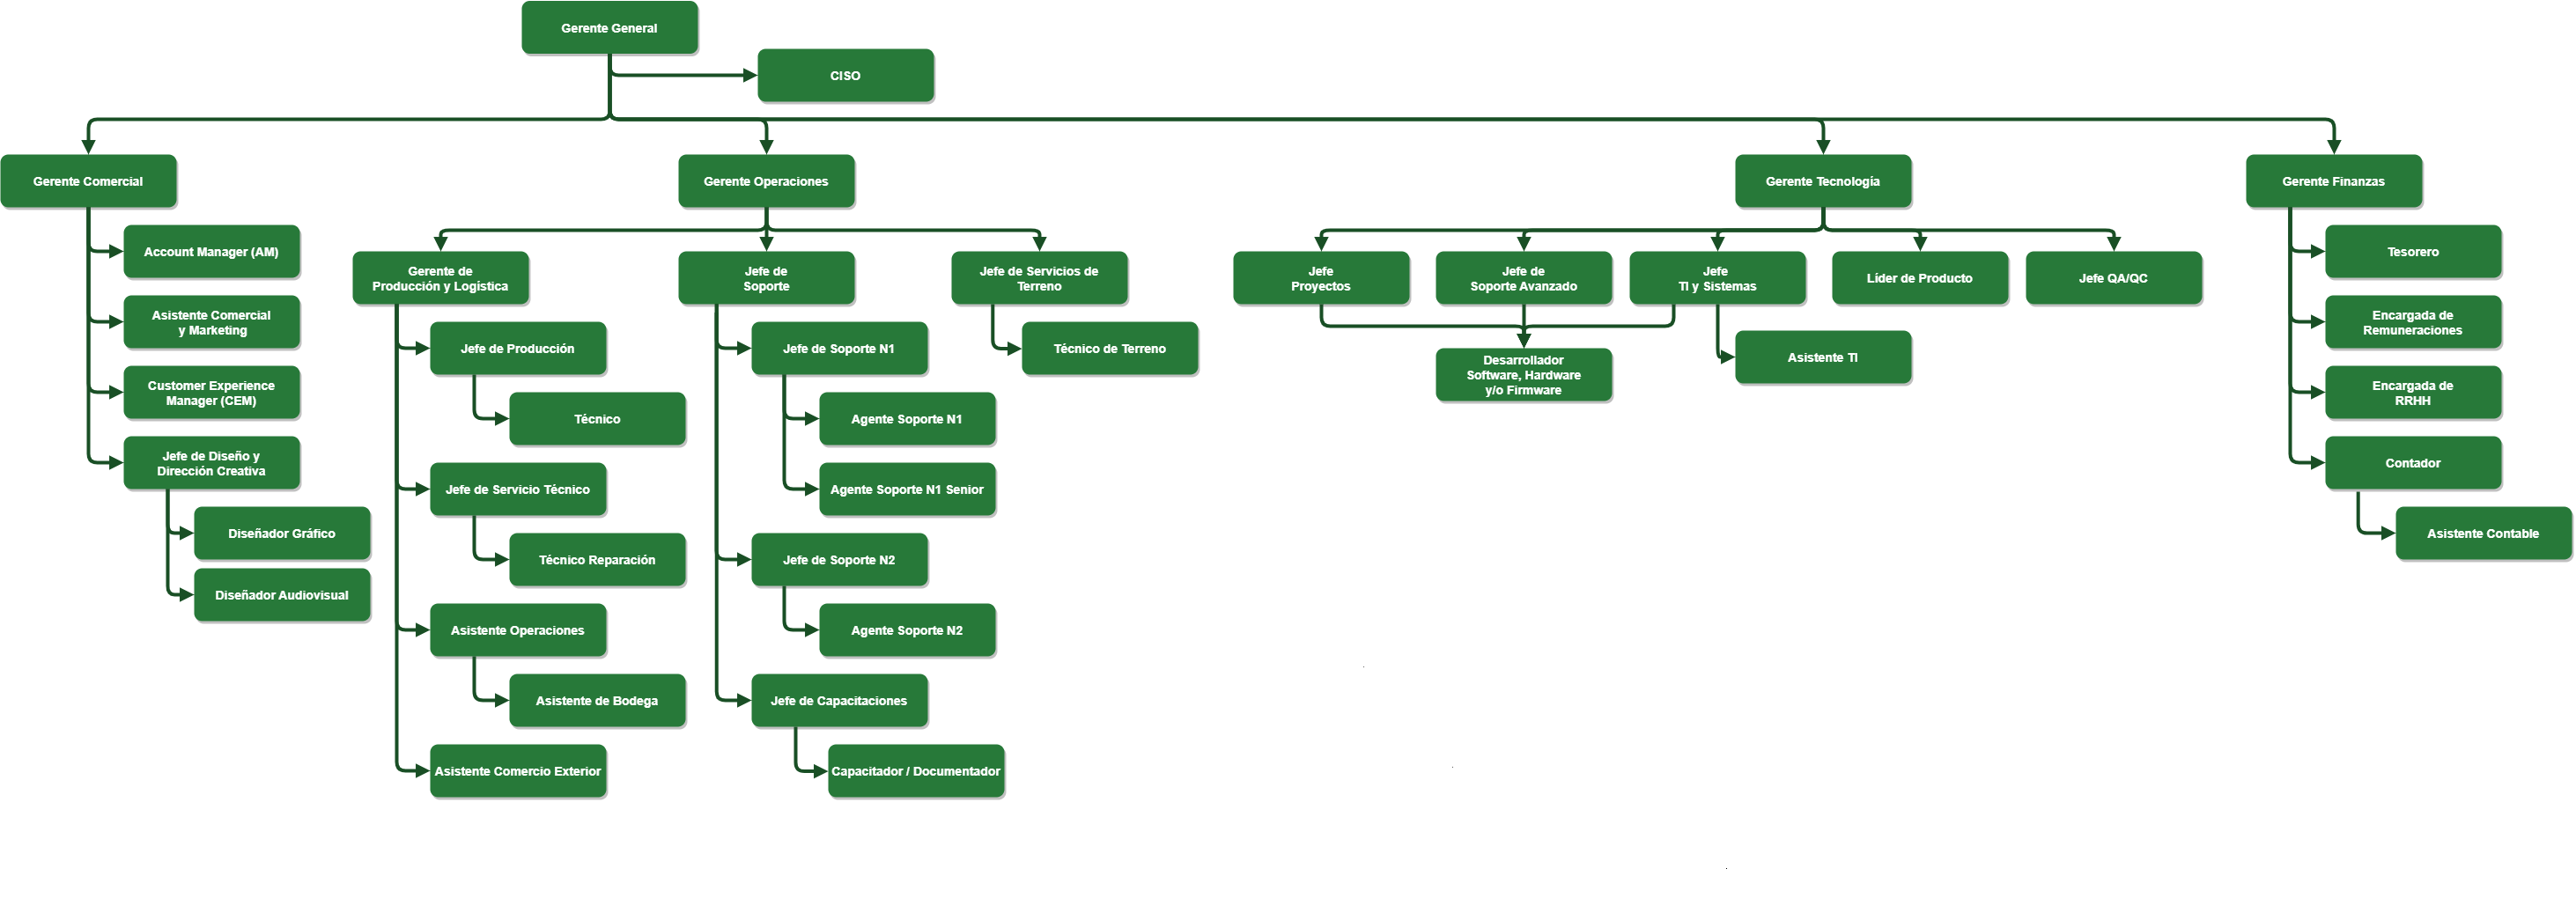
\includegraphics[width=0.8\textwidth]{Organigrama_WiseConn}
	\caption{\label{fig:orgwis} Organigrama de Wiseconn}
\end{figure}

\subsection{PRODUCTOS}
\subsubsection{HARDWARE}

El hardware ha sido especialmente diseñado por la empresa para el monitoreo y control de riego, los componentes principales son los nodos, dispositivos de monitoreo y control IoT que operan en terreno y se comunican mediante radio y celular para conectarse a la nube. Existen 3 modelos, los cuales se diferencian según si se quiere realizar un simple monitoreo, control en terreno o control completo sobre los componentes de un sistema de riego.
\begin{itemize}
	\item \textbf{RF-M1:} Nodo de monitoreo de campo. Permite obtener información de variables agroclimáticas, variables de suelo, sensores de riego y variables de planta.
	\item \textbf{RF-X1:} Nodo de monitoreo y control de campo. Permite el control y monitoreo de válvulas, monitoreo de campo, control de la estación de bombeo, control de fertirriego, control PID y automatización remota.
	\item \textbf{RF-C1:} Nodo de control de caseta de riego. Permite el control y monitoreo de casetas de riego, válvulas, retrolavados e inyección de fertilizantes y pH, monitoreo y control de variadores de frecuencia y automatización industrial remota.
\end{itemize}

\subsubsection{SOFTWARE}
Wiseconn ofrece Software como Servicio o SaaS (del inglés, Software as a Service), ya que, estos se acceden mediante la web sin necesidad de instalación previa. Estos servicios ofrecen el almacenamiento y visualización de información recolectada en terreno y poder configurar los componentes de una manera óptima y sin complicaciones. Los softwares que ofrecen son:
\begin{itemize}
    \item \textbf{DropControl:} Es una plataforma online que permite el monitoreo de control y riego/fertirriego avanzado, capaz de conectarse con cualquier sensor, equipo de riego y fertilización de manera simple y confiable.
    \item \textbf{Aplicación Móvil:} Plataforma móvil enfocada para los operadores en terreno, monitoreo y control de riego, monitoreo de variables, informes calicatas, notificaciones de alarmas.
    \item \textbf{Admin de DropControl:} Servicio enfocado a los usuarios administradores de campo para realizar modificaciones de sectores de riego, usuarios, servicios API, entre otros.
\end{itemize}

Para estos servicios se ofrecen planes, cuyos factores diferenciales son esencialmente herramientas especializadas, el acceso a la aplicación web y/o móvil, cantidad de usuarios permitidos, almacenamiento, acceso a funcionalidades, entre otros.
Wiseconn también tiene software interno utilizado por trabajadores de distintas áreas de la empresa como soporte y producción, para hacer configuraciones avanzadas de campos o temas productivos como manejo de inventarios, lotes, despachos, etc. Dentro de estos softwares están:
\begin{itemize}
    \item \textbf{Operations:} Plataforma para la gestión de lotes y despacho de productos.
    \item \textbf{Setup:} Plataforma de configuración paso a paso. Provee herramientas de gestión para cuentas, campos y usuarios con el fin de crear y organizar los permisos a usar en DropControl o en el mismo Setup.
\end{itemize}

\subsection{SITUACIÓN ACTUAL}

\subsubsection{DESCRIPCIÓN}
En la actualidad, el usuario cliente no tiene completo acceso a realizar ciertas configuraciones en los campos, para esto se tiene que recurrir al área de soporte mandando un ticket con la configuración a realizar. Algunas de estas configuraciones son procesos que consumen mucho tiempo y esfuerzo para los trabajadores de soporte. Esto puede significar una carga innecesaria y/o un aumento en el personal para poder llevar a cabo estos procesos en un tiempo razonable. Por el lado del usuario cliente, genera un descontento debido a la alta espera por la configuración.
En los procesos productivos, las herramientas de softwares son limitadas y los trabajadores deben hacer pasos extras innecesarios para poder realizar la tarea correspondiente. Debido a esto, puede haber algunos errores y retrasos en producción.
Como se explicó anteriormente, Wiseconn ofrece planes gratuitos y de pago. En el caso del plan gratuito, este habilita un punto de entrada para aquellos usuarios que no están dispuestos a realizar pagos recurrentes. Sin embargo, existen limitaciones para el usuario cliente debido a la baja cantidad de funcionalidades y/o herramientas disponibles, lo que impide poder entregar condiciones mínimas al usuario que cumplan con las especificaciones comerciales. Además, puede influir en la poca retención de usuarios y/o que estos no se cambien a un plan de pago.

\subsubsection{ACTORES}
Dentro de los actores que podemos encontrar es, primero, el usuario cliente que utiliza y/o paga los servicios que ofrece Wiseconn para la gestión de riego de sus campos. Segundo, los trabajadores de Wiseconn del área de soporte y producción que utilizan los softwares internos para la realización de sus respectivas tareas.

\subsubsection{ÁRBOL DEL PROBLEMA}
En la figura \ref{fig:arbolproblema} se encuentra representado el árbol del problema, que identifica como problema principal es que el software de Wiseconn tiene funcionalidades limitadas y con harta intervención humana.
En la parte inferior se presentan las causas como que el usuario depende del área de soporte para la realización de algunas configuraciones, el plan gratuito no cumple con las especificaciones comerciales mínimas y, por último, procesos que consumen mucho tiempo y esfuerzo para los trabajadores.
En la parte superior, se presentan los efectos que puede generar este problema como el aumento en la posibilidad de errores, retrasos en producción, usuario final descontento por la espera de las configuraciones, el usuario no cambia al plan de pago o cancela sus servicios y mayor carga en el área de soporte.

\begin{figure}
    \centering
	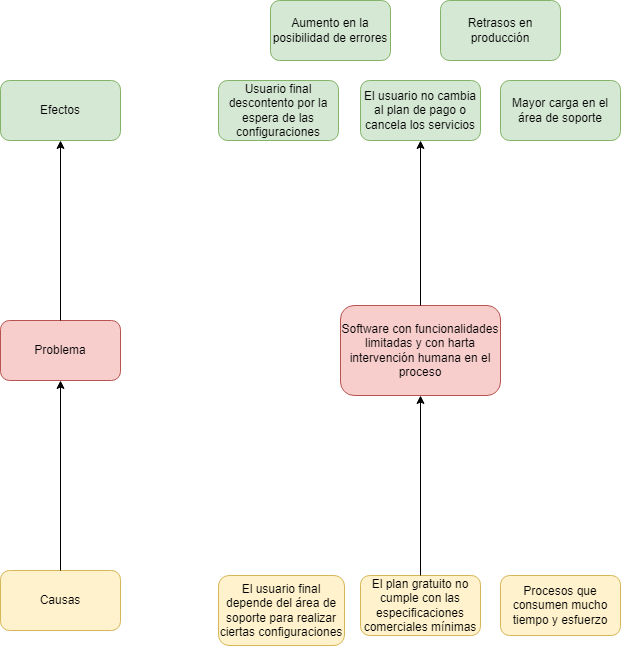
\includegraphics[width=0.8\textwidth]{arbol del problema}
	\caption{\label{fig:arbolproblema} Árbol del problema} Fuente: Elaboración propia.
\end{figure}

\subsection{SOLUCIÓN}

\subsubsection{OBJETIVO GENERAL}

Análisis, diseño e implementación de herramientas de software que faciliten tareas a usuarios y mejoren procesos para un escalamiento global de servicios de WiseConn, para así, poder reducir tiempo y esfuerzo en los trabajadores de distintas áreas de la empresa, como también, reducir la brecha asociadas a los cobros de servicios SaaS.

\subsubsection{OBJETIVOS ESPECÍFICOS}
\begin{itemize}
    \item Hacer un análisis de los procesos de producción que más cargan y esfuerzo generan, como también de funcionalidades/herramientas necesarias para el plan gratuito.
    \item A partir del análisis previo, diseñar las herramientas de software correspondientes para los servicios de WiseConn.
    \item Implementación de las herramientas de software en los servicios de WiseConn correspondientes.
\end{itemize}

\subsubsection{ALCANCE DE LA SOLUCIÓN}
Al finalizar esta memoria se espera reducir los tiempos y esfuerzos en las áreas de soporte y producción de la empresa, ya sea, mejorando herramientas internas o transfiriendo tareas/procesos al usuario cliente. También, ayudar a reducir la brecha de cobros en servicios SaaS con alternativas gratuitas de ciertas funcionalidades, lo que permitiría que el plan gratuito de Wiseconn cumpla con las especificaciones comerciales.
